% PRL look and style (easy on the eyes)
%\RequirePackage[hyphens]{url}
%\documentclass[linenumbers,11point]{achemso}
\documentclass[aps,pre,twocolumn,nofootinbib,superscriptaddress,linenumbers,11point]{revtex4-1}
% Two-column style (for submission/review/editing)
%\documentclass[aps,prl,preprint,nofootinbib,superscriptaddress,linenumbers]{revtex4-1}

%\usepackage{palatino}

% Change to a sans r font.
\usepackage{sourcesanspro}
\renewcommand*\familydefault{\sfdefault} %% Only if the base font of the document is to be sans serif
\usepackage[T1]{fontenc}
%\usepackage[font=sf,justification=justified]{caption}
%\usepackage[font=sf]{floatrow}

% Rework captions to use sans serif font.
\makeatletter
\renewcommand\@make@capt@title[2]{%
 \@ifx@empty\float@link{\@firstofone}{\expandafter\href\expandafter{\float@link}}%
  {\textbf{#1}}\sf\@caption@fignum@sep#2\quad
}%
\makeatother

\usepackage{listings} % For code examples
\usepackage[usenames,dvipsnames,svgnames,table]{xcolor}

\usepackage{minted}

\usepackage{amsmath}
\usepackage{amssymb}
\usepackage{graphicx}
%\usepackage[mathbf,mathcal]{euler}
%\usepackage{citesort}
\usepackage{dcolumn}
\usepackage{boxedminipage}
\usepackage{verbatim}
\usepackage[colorlinks=true,citecolor=blue,linkcolor=blue]{hyperref}
%\usepackage[colorlinks=false,citecolor=blue,linkcolor=blue]{hyperref}

\usepackage{subfigure}  % use for side-by-side figures

% The figures are in a figures/ subdirectory.
\graphicspath{{figures/}}

% italicized boldface for math (e.g. vectors)
\newcommand{\bfv}[1]{{\mbox{\boldmath{$#1$}}}}
% non-italicized boldface for math (e.g. matrices)
\newcommand{\bfm}[1]{{\bf #1}}          

%\newcommand{\bfm}[1]{{\mbox{\boldmath{$#1$}}}}
%\newcommand{\bfm}[1]{{\bf #1}}
%\newcommand{\expect}[1]{\left \langle #1 \right \rangle}                % <.> for denoting expectations over realizations of an experiment or thermal averages

% Define some useful commands we will use repeatedly.
\newcommand{\T}{\mathrm{T}}                                % T used in matrix transpose
\newcommand{\tauarrow}{\stackrel{\tau}{\rightarrow}}       % the symbol tau over a right arrow
\newcommand{\expect}[1]{\langle #1 \rangle}                % <.> for denoting expectations over realizations of an experiment or thermal averages
\newcommand{\estimator}[1]{\hat{#1}}                       % estimator for some quantity from a finite dataset.
\newcommand{\code}[1]{{\tt #1}}

% vectors
\newcommand{\x}{\bfv{x}}
\newcommand{\y}{\bfv{y}}
\newcommand{\f}{\bfv{f}}

\newcommand{\bfc}{\bfm{c}}
\newcommand{\hatf}{\hat{f}}

%\newcommand{\bTheta}{\bfm{\Theta}}
%\newcommand{\btheta}{\bfm{\theta}}
%\newcommand{\bhatf}{\bfm{\hat{f}}}
%\newcommand{\Cov}[1] {\mathrm{cov}\left( #1 \right)}
%\newcommand{\Ept}[1] {{\mathrm E}\left[ #1 \right]}
%\newcommand{\Eptk}[2] {{\mathrm E}\left[ #2 \,|\, #1\right]}
%\newcommand{\T}{\mathrm{T}}                                % T used in matrix transpose
%\newcommand{\conc}[1] {\left[ \mathrm{#1} \right]}

\DeclareMathOperator*{\argmin}{argmin}
\DeclareMathOperator*{\argmax}{argmax}
\newcommand*{\argminl}{\argmin\limits}
\newcommand*{\argmaxl}{\argmax\limits}

%%%%%%%%%%%%%%%%%%%%%%%%%%%%%%%%%%%%%%%%%%%%%%%%%%%%%%%%%%%%%%%%%%%%%
%% Meta-data block
%% ---------------
%% Each author should be given as a separate \author command.
%%
%% Corresponding authors should have an e-mail given after the author
%% name as an \email command. Phone and fax numbers can be given
%% using \phone and \fax, respectively; this information is optional.
%%
%% The affiliation of authors is given after the authors; each
%% \affiliation command applies to all preceding authors not already
%% assigned an affiliation.
%%
%% The affiliation takes an option argument for the short name.  This
%% will typically be something like "University of Somewhere".
%%
%% The \altaffiliation macro should be used for new address, etc.
%% On the other hand, \alsoaffiliation is used on a per author basis
%% when authors are associated with multiple institutions.
%%%%%%%%%%%%%%%%%%%%%%%%%%%%%%%%%%%%%%%%%%%%%%%%%%%%%%%%%%%%%%%%%%%%%

%\author{John D. Chodera}
% \email{john.chodera@choderalab.org}
% \affiliation{Computational Biology Program, Sloan Kettering Institute, Memorial Sloan Kettering Cancer Center, New York, NY 10065}
%
%%%%%%%%%%%%%%%%%%%%%%%%%%%%%%%%%%%%%%%%%%%%%%%%%%%%%%%%%%%%%%%%%%%%%%
%%% The document title should be given as usual. Some journals require
%%% a running title from the author: this should be supplied as an
%%% optional argument to \title.
%%%%%%%%%%%%%%%%%%%%%%%%%%%%%%%%%%%%%%%%%%%%%%%%%%%%%%%%%%%%%%%%%%%%%%
%\title[Automated equilibration detection]
%  {A simple method for automated equilibration detection in molecular simulations}
%
%%%%%%%%%%%%%%%%%%%%%%%%%%%%%%%%%%%%%%%%%%%%%%%%%%%%%%%%%%%%%%%%%%%%%%
%%% Some journals require a list of abbreviations or keywords to be
%%% supplied. These should be set up here, and will be printed after
%%% the title and author information, if needed.
%%%%%%%%%%%%%%%%%%%%%%%%%%%%%%%%%%%%%%%%%%%%%%%%%%%%%%%%%%%%%%%%%%%%%%
%\abbreviations{MD,MC,MCMC}
%\keywords{molecular dynamics (MD); Metropolis-Hastings; Monte Carlo (MC); Markov chain Monte Carlo (MCMC); equilibration; burn-in; timeseries analysis; statistical inefficiency; integrated autocorrelation time}
%
%%%%%%%%%%%%%%%%%%%%%%%%%%%%%%%%%%%%%%%%%%%%%%%%%%%%%%%%%%%%%%%%%%%%%%%%%%%%%%%%%
%% DOCUMENT
%%%%%%%%%%%%%%%%%%%%%%%%%%%%%%%%%%%%%%%%%%%%%%%%%%%%%%%%%%%%%%%%%%%%%%%%%%%%%%%%%
%
%\begin{document}
%
%%%%%%%%%%%%%%%%%%%%%%%%%%%%%%%%%%%%%%%%%%%%%%%%%%%%%%%%%%%%%%%%%%%%%%
%%% The "tocentry" environment can be used to create an entry for the
%%% graphical table of contents. It is given here as some journals
%%% require that it is printed as part of the abstract page. It will
%%% be automatically moved as appropriate.
%%%%%%%%%%%%%%%%%%%%%%%%%%%%%%%%%%%%%%%%%%%%%%%%%%%%%%%%%%%%%%%%%%%%%%
%\begin{tocentry}
%
%\begin{centering}
%\resizebox{9cm}{!}{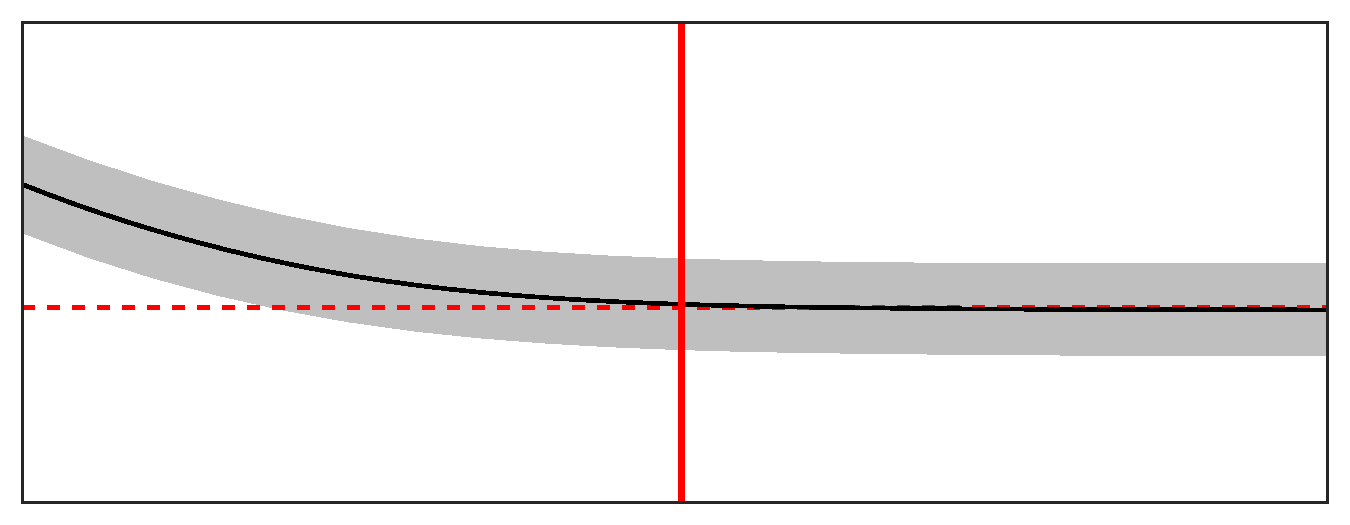
\includegraphics{toc-graphic.pdf}}
%
%\end{centering}
%%
%%Some journals require a graphical entry for the Table of Contents.
%%This should be laid out ``print ready'' so that the sizing of the
%%text is correct.
%%
%%Inside the \texttt{tocentry} environment, the font used is Helvetica
%%8\,pt, as required by \emph{Journal of the American Chemical
%%Society}.
%%
%%The surrounding frame is 9\,cm by 3.5\,cm, which is the maximum
%%permitted for  \emph{Journal of the American Chemical Society}
%%graphical table of content entries. The box will not resize if the
%%content is too big: instead it will overflow the edge of the box.
%%
%%This box and the associated title will always be printed on a
%%separate page at the end of the document.
%
%\end{tocentry}
%
%%%%%%%%%%%%%%%%%%%%%%%%%%%%%%%%%%%%%%%%%%%%%%%%%%%%%%%%%%%%%%%%%%%%%%%%%%%%%%%%%
%% ABSTRACT
%%%%%%%%%%%%%%%%%%%%%%%%%%%%%%%%%%%%%%%%%%%%%%%%%%%%%%%%%%%%%%%%%%%%%%%%%%%%%%%%%
%
%\begin{abstract}
%
%Molecular simulations intended to compute equilibrium properties are often initiated from configurations that are highly atypical of equilibrium samples, a practice which can generate a distinct initial transient in mechanical observables computed from the simulation trajectory.
%Traditional practice in simulation data analysis recommends this initial portion be discarded to \emph{equilibration}, but no simple, general, and automated procedure for this process exists.
%Here, we suggest a conceptually simple automated procedure that does not make strict assumptions about the distribution of the observable of interest, in which the equilibration time is chosen to maximize the number of effectively uncorrelated samples in the production timespan used to compute equilibrium averages.
%We present a simple Python reference implementation of this procedure, and demonstrate its utility on typical molecular simulation data.\\
%
%% KEYWORDS
%\emph{Keywords: molecular dynamics (MD); Metropolis-Hastings; Monte Carlo (MC); Markov chain Monte Carlo (MCMC); equilibration; burn-in; timeseries analysis; statistical inefficiency; integrated autocorrelation time}
%
%\end{abstract}
%
%\maketitle

%%%%%%%%%%%%%%%%%%%%%%%%%%%%%%%%%%%%%%%%%%%%%%%%%%%%%%%%%%%%%%%%%%%%%%%%%%%%%%%%
% DOCUMENT
%%%%%%%%%%%%%%%%%%%%%%%%%%%%%%%%%%%%%%%%%%%%%%%%%%%%%%%%%%%%%%%%%%%%%%%%%%%%%%%%

\begin{document}

%%%%%%%%%%%%%%%%%%%%%%%%%%%%%%%%%%%%%%%%%%%%%%%%%%%%%%%%%%%%%%%%%%%%%%%%%%%%%%%%
% TITLE
%%%%%%%%%%%%%%%%%%%%%%%%%%%%%%%%%%%%%%%%%%%%%%%%%%%%%%%%%%%%%%%%%%%%%%%%%%%%%%%%

\title{A simple method for automated equilibration detection in molecular simulations}

\author{John D. Chodera}
 \thanks{Corresponding author}
 \email{john.chodera@choderalab.org}
 \affiliation{Computational Biology Program, Sloan Kettering Institute, Memorial Sloan Kettering Cancer Center, New York, NY 10065}

\date{\today}

%%%%%%%%%%%%%%%%%%%%%%%%%%%%%%%%%%%%%%%%%%%%%%%%%%%%%%%%%%%%%%%%%%%%%%%%%%%%%%%%
% ABSTRACT
%%%%%%%%%%%%%%%%%%%%%%%%%%%%%%%%%%%%%%%%%%%%%%%%%%%%%%%%%%%%%%%%%%%%%%%%%%%%%%%%

\begin{abstract}

Molecular simulations intended to compute equilibrium properties are often initiated from configurations that are highly atypical of equilibrium samples, a practice which can generate a distinct initial transient in mechanical observables computed from the simulation trajectory.
Traditional practice in simulation data analysis recommends this initial portion be discarded to \emph{equilibration}, but no simple, general, and automated procedure for this process exists.
Here, we suggest a conceptually simple automated procedure that does not make strict assumptions about the distribution of the observable of interest, in which the equilibration time is chosen to maximize the number of effectively uncorrelated samples in the production timespan used to compute equilibrium averages.
We present a simple Python reference implementation of this procedure, and demonstrate its utility on typical molecular simulation data.\\

% KEYWORDS
\emph{Keywords: molecular dynamics (MD); Metropolis-Hastings; Monte Carlo (MC); Markov chain Monte Carlo (MCMC); equilibration; burn-in; timeseries analysis; statistical inefficiency; integrated autocorrelation time}

\end{abstract}

\maketitle

%%%%%%%%%%%%%%%%%%%%%%%%%%%%%%%%%%%%%%%%%%%%%%%%%%%%%%%%%%%%%%%%%%%%%%%%%%%%%%%%
% FIGURE: BURN-IN EXAMPLE
%%%%%%%%%%%%%%%%%%%%%%%%%%%%%%%%%%%%%%%%%%%%%%%%%%%%%%%%%%%%%%%%%%%%%%%%%%%%%%%%

\begin{figure*}[tbp]
\resizebox{0.9\textwidth}{!}{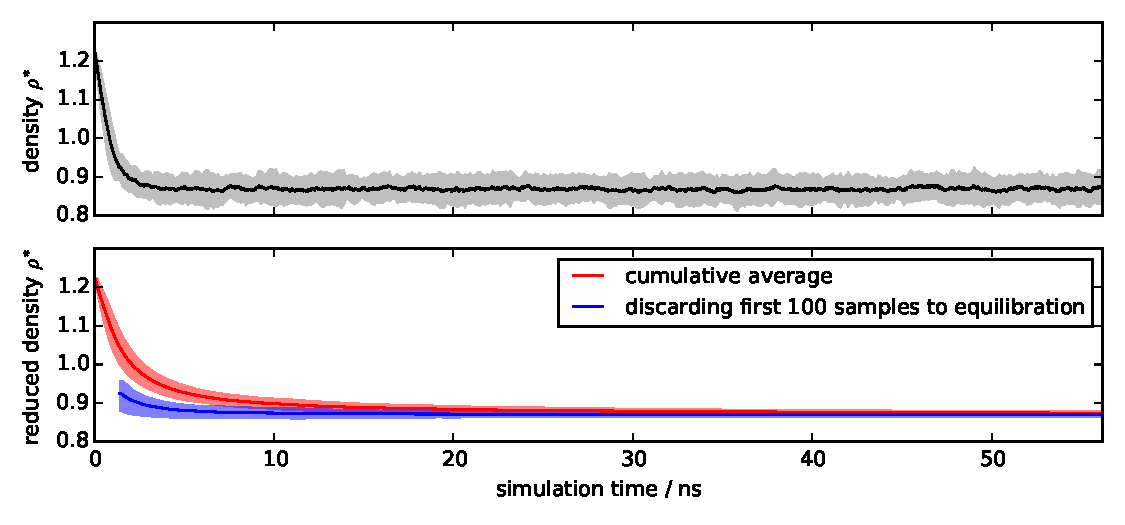
\includegraphics{argon-density.pdf}}
\caption{\label{figure:burn-in-example} {\bf Illustration of the motivation for discarding data to equilibration.} 
To illustrate the bias in expectations induced by relaxation away from initial conditions, 500 replicates of a simulation of liquid argon were initiated from the same energy-minimized initial configuration constructed with initial reduced density $\rho^* \equiv \rho \sigma^3 = 0.960$ but different random number seeds for stochastic integration.
%
{\bf Top:} The average of the reduced density (black line) over the replicates relaxes to the region of typical equilibrium densities over the first $\sim 100~\tau$ of simulation time, where $\tau$ is a natural time unit (see \emph{Simulation Details}).
%
{\bf Bottom:} If the average density is estimated by a cumulative average from the beginning of the simulation (red dotted line), the estimate will be heavily biased by the atypical starting density even beyond $1000~\tau$.
Discarding even a small amount of initial data---in this case 500 initial samples---results in a cumulative average estimate that converges to the true average (black dashed line) much more rapidly.
% 
Shaded regions denote 95\% confidence intervals.
}
\end{figure*}

%%%%%%%%%%%%%%%%%%%%%%%%%%%%%%%%%%%%%%%%%%%%%%%%%%%%%%%%%%%%%%%%%%%%%%%%%%%%%%%%
% INTRODUCTION
%%%%%%%%%%%%%%%%%%%%%%%%%%%%%%%%%%%%%%%%%%%%%%%%%%%%%%%%%%%%%%%%%%%%%%%%%%%%%%%%

\section*{Introduction}
\label{section:introduction}

Molecular simulations use Markov chain Monte Carlo (MCMC) techniques~\cite{jun-s-liu:mcmc} to sample configurations $x$ from an equilibrium distribution $\pi(x)$, either exactly (using Monte Carlo methods such as Metropolis-Hastings) or approximately (using molecular dynamics integrators without Metropolization)~\cite{sivak:2013:prx:vvvr}.

Due to the sensitivity of the equilibrium probability density $\pi(x)$ to small perturbations in configuration $x$ and the difficulty of producing sufficiently good guesses of typical equilibrium configurations $x \sim \pi(x)$, these molecular simulations are often started from highly atypical initial conditions.
For example, simulations of biopolymers might be initiated from a fully extended conformation unrepresentative of behavior in solution, or a geometry derived from a fit to diffraction data collected from a cryocooled crystal; 
solvated systems may be prepared by periodically replicating a small solvent box equilibrated under different conditions, yielding atypical densities and solvent structure; 
liquid mixtures or lipid bilayers may be constructed by using methods that fulfill spatial constraints (e.g.~PackMol~\cite{martinez:jctc:2009:packmol}) but create locally aytpical geometries, requiring long simulation times to relax to typical configurations.

As a result, traditional practice in molecular simulation has recommended some initial portion of the trajectory be discarded to \emph{equilibration} (also called \emph{burn-in}\footnote{The term \emph{burn-in} comes from the field of electronics, in which a short ``burn-in'' period is used to ensure that a device is free of faulty components---which often fail quickly---and is operating normally~\cite{crc-mcmc-handbook}.} in the MCMC literature~\cite{crc-mcmc-handbook}).
While the process of discarding initial samples is strictly unnecessary for the time-average of quantities of interest to eventually converge to the desired expectations~\cite{geyer:burn-in-unnecessary}, this nevertheless often allows the practitioner to avoid what may be impractically long run times to eliminate the bias in computed properties in finite-length simulations induced by atypical initial starting conditions.
It is worth noting that a similar procedure is not a practice universally recommended by statisticians when sampling from posterior distributions in statistical inference~\cite{crc-mcmc-handbook}; the differences in complexity of probability densities typically encountered in statistics and molecular simulation may explain the difference in historical practice.

% Liquid argon example
% JDC: Should we use TIP3P water instead?
As a motivating example, consider the computation of the average density of liquid argon under a given set of reduced temperature and pressure conditions shown in Figure~\ref{figure:burn-in-example}.
To initiate the simulation, an initial dense liquid geometry at reduced density $\rho^* \equiv \rho \sigma^3 = 0.960$ was prepared and subjected to local energy minimization.
The upper panel of Figure~\ref{figure:burn-in-example} depicts the average relaxation behavior of simulations initiated from the same configuration with different random initial velocities and integrator random number seeds (see \emph{Simulation Details}).
The average of 500 realizations of this process shows a characteristic relaxation away from the initial density toward the equilibrium density (Figure~\ref{figure:burn-in-example}, upper panel, black line).
As a result, the expectation of the running average of the density significantly deviates from the true expectation (Figure~\ref{figure:burn-in-example}, lower panel, dashed line).
This effect leads to significantly biased estimates of the expectation unless simulations are sufficiently long to eliminate starting point dependent bias, which takes a surprisingly long $\sim$2000$\tau$ in this example.
Note that this bias is present even in the average of many realizations because the \emph{same} atypical starting condition is used for every realization of this simulation process.

To develop an automatic approach to eliminating this bias, we take motivation from the concept of \emph{reverse cumulative averaging} from Yang et al.~\cite{yang-karplus:2004:jcp:reverse-cumulative-averaging}, in which the trajectory statistics over the production region of the trajectory are examined for different choices of the end of the discarded equilibration region to determine the optimal production region to use for computing expectations and other statistical properties.
We begin by first formalizing our objectives mathematically.

%%%%%%%%%%%%%%%%%%%%%%%%%%%%%%%%%%%%%%%%%%%%%%%%%%%%%%%%%%%%%%%%%%%%%%%%%%%%%%%%
% FIGURE: BURN-IN EXAMPLE
%%%%%%%%%%%%%%%%%%%%%%%%%%%%%%%%%%%%%%%%%%%%%%%%%%%%%%%%%%%%%%%%%%%%%%%%%%%%%%%%

\begin{figure*}[tbp]
\resizebox{0.9\textwidth}{!}{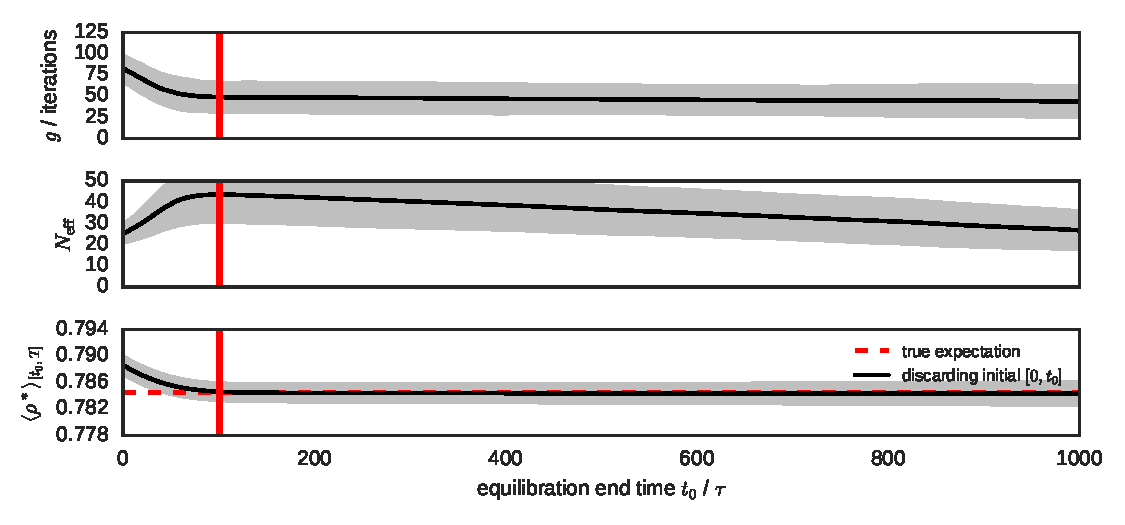
\includegraphics{argon-reverse-cumulative-average.pdf}}
\caption{\label{figure:reverse-cumulative-average} {\bf Statistical inefficiency, number of uncorrelated samples, and bias for different equilibration times.} 
Trajectories of length $T = 2000~\tau$ for the argon system described in Figure~\ref{figure:burn-in-example} were analyzed as a function of equilibration time choice $t_0$.
Averages over all 500 replicate simulations (all starting from the same initial conditions) are shown as dark lines, with shaded lines showing standard deviation of estimates among replicates.
{\bf Top:} The statistical inefficiency $g$ as a function of equilibration time choice $t_0$ is initially very large, but diminishes rapidly after the system has relaxed to equilibrium.
{\bf Middle:} The number of effectively uncorrelated samples $N_\mathrm{eff} = (T - t_0 + 1) / g$ shows a maximum at $t_0 \sim 100~\tau$ (red vertical lines), suggesting the system has equilibrated by this time.
{\bf Bottom:} The cumulative average density $\expect{\rho^*}$ computed over the span $[t_0, T]$ shows that the bias (deviation from the true estimate, shown as red dashed lines) is minimized for choices of $t_0 \ge 100~\tau$.
The standard deviation among replicates (shaded region) grows with $t_0$ because fewer data are included in the estimate.
The choice of optimal $t_0$ that maximizes $N_\mathrm{eff}$ (red vertical line) strikes a good balance between bias and variance.
The true estimate (red dashed lines) is computed from averaging over the range [5~000, 10~000] $\tau$ over all 500 replicates.
}
\end{figure*}

%%%%%%%%%%%%%%%%%%%%%%%%%%%%%%%%%%%%%%%%%%%%%%%%%%%%%%%%%%%%%%%%%%%%%%%%%%%%%%%%
% STATEMENT OF THE PROBLEM
%%%%%%%%%%%%%%%%%%%%%%%%%%%%%%%%%%%%%%%%%%%%%%%%%%%%%%%%%%%%%%%%%%%%%%%%%%%%%%%%

\section*{Statement of the problem}

Consider $T$ successively sampled configurations $x_t$ from a molecular simulation, with $t = 1, \ldots, T$, initiated from $x_0$.
We presume we are interested in computing the expectation
\begin{eqnarray}
\expect{A} \equiv \int dx \, A(x) \, \pi(x)
\end{eqnarray}
of a mechanical property of interest $A(x)$.
For convenience, we will refer to the timeseries $a_t \equiv A(x_t)$, with $t \in [1,T]$.
The estimator $\hat{A} \approx \expect{A}$ constructed from the entire dataset is given by
\begin{eqnarray}
\hat{A}_{[1,T]} \equiv \frac{1}{T} \sum_{t=1}^T a_t . \label{equation:time-average}
\end{eqnarray}
While $\lim_{T \rightarrow \infty} \hat{A}_{[1,T]} = \expect{A}$ for an infinitely long simulation\footnote{We note that this equality only holds for simulation schemes that sample from the true equilibrium density $\pi(x)$, such as Metropolis-Hastings Monte Carlo or Metropolized dynamical integration schemes such as hybrid Monte Carlo (HMC). Molecular dynamics simulations utilizing finite timestep integration without Metropolization will produce averages that may deviate from the true expectation $\expect{A}$~\cite{sivak:2013:prx:vvvr}.}, the bias in $\hat{A}_{[1,T]}$ may be significant in a simulation of finite length $T$.

By discarding samples $t < t_0$ to equilibration, we hope to exclude the initial transient from our sample average, and provide a less biased estimate of $\expect{A}$,
\begin{eqnarray}
\hat{A}_{[t_0,T]} \equiv \frac{1}{T-t_0+1} \sum_{t=t_0}^T a_t . \label{equation:production-time-average} 
\end{eqnarray}

We can quantify the overall error in an estimator $\hat{A}_{[t_0,T]}$ in a sample average of trajectories initiated from $x_0$ that excludes samples where $t < t_0$ by the expected error $\delta^2 \hat{A}_{[t_0,T]}$,
\begin{eqnarray}
\delta^2 \hat{A}_{[t_0,T]} &\equiv& E_{x_0} \left[ \left( \hat{A}_{[t_0,T]} - \expect{A} \right)^2 \right] \label{equation:rms-error} 
\end{eqnarray}
where $E_{x_0}[\cdot]$ denotes the expectation over independent realizations of the specific simulation process initiated from configuration $x_0$, but with different velocities and random number seeds.

We can rewrite the expected error $\delta^2 \hat{A}$ by separating it into two components:
\begin{eqnarray}
\delta^2 \hat{A}_{[t_0,T]} = E_{x_0}\left[ \left( \hat{A}_{[t_0,T]} - E_{x_0}[\hat{A}_{[t_0,T]}] \right)^2 \right] \nonumber \\
+ \left( E_{x_0}[\hat{A}_{[t_0,T]}] - \expect{A} \right)^2  \label{equation:bias-variance}  
\end{eqnarray}
The first term denotes the variance in the estimator $\hat{A}$,
\begin{eqnarray}
\mathrm{var}_{x_0} (\hat{A}_{[t_0,T]}) &\equiv& E_{x_0} \left[ \left( \hat{A}_{[t_0,T]} - E_{x_0}[\hat{A}_{[t_0,T]}]\right)^2 \right] \label{equation:variance}
\end{eqnarray}
while the second term denotes the contribution from the squared bias,
\begin{eqnarray}
\mathrm{bias}^2_{x_0} (\hat{A}_{[t_0,T]}) &\equiv& \left( E_{x_0}[\hat{A}_{[t_0,T]}] - \expect{A} \right)^2 \label{equation:variance}
\end{eqnarray}

%%%%%%%%%%%%%%%%%%%%%%%%%%%%%%%%%%%%%%%%%%%%%%%%%%%%%%%%%%%%%%%%%%%%%%%%%%%%%%%%
% BIAS-VARIANCE TRADEOFF
%%%%%%%%%%%%%%%%%%%%%%%%%%%%%%%%%%%%%%%%%%%%%%%%%%%%%%%%%%%%%%%%%%%%%%%%%%%%%%%%

\section*{Bias-variance tradeoff}

With increasing equilibration time $t_0$, bias is reduced, but the variance---the contribution to error due to random variation from having a finite number of uncorrelated samples---will increase because less data is included in the estimate.
This can be seen in the bottom panel of Figure~\ref{figure:reverse-cumulative-average}, where the shaded region (95\% confidence interval of the mean) increases in width with increasing equilibration time $t_0$.

To examine the tradeoff between bias and variance explicitly, Figure~\ref{figure:bias-variance} plots the bias and variance (here, shown as the standard deviation over replicates---the square root of the variance---which is an indication of the true standard error of a single simulation) contributions against each other as a function of $t_0$ (denoted by color) as computed from statistics over all 500 replicates.
At $t_0 = 0$, the bias is large but variance is minimized.
With increasing $t_0$, bias is eventually eliminated but then variance rapidly grows as fewer uncorrelated samples are included in the estimate.
There is a clear optimal choice at $t_0 \sim 100~\tau$ that minimizes variance while also effectively eliminating bias (where $\tau$ is a natural time unit---see \emph{Simulation Details}).

%%%%%%%%%%%%%%%%%%%%%%%%%%%%%%%%%%%%%%%%%%%%%%%%%%%%%%%%%%%%%%%%%%%%%%%%%%%%%%%%
% BIAS-VARIANCE TRADEOFF
%%%%%%%%%%%%%%%%%%%%%%%%%%%%%%%%%%%%%%%%%%%%%%%%%%%%%%%%%%%%%%%%%%%%%%%%%%%%%%%%

\section*{Selecting the equilibration time}

Is there a simple approach to choosing an optimal equilibration time $t_0$ that provides a significantly improved estimate $\hat{A}_{[t_0,T]}$, even when we do not have access to multiple realizations?
At worst, we hope that such a procedure would at least give some improvement over the naive estimate, such that $\delta^2 \hat{A}_{[t_0,T]} < \delta^2 \hat{A}_{[0,T]}$; at best, we hope that we can achieve a reasonable bias-variance tradeoff close to the optimal point identified in Figure~\ref{figure:bias-variance} that minimizes bias without greatly increasing variance.
We remark that, for cases in which the simulation is not long enough to reach equilibrium, no choice of $t_0$ will eliminate bias completely; the best we can hope for is to minimize this bias.

While automated methods for selecting the equilibration time $t_0$ have been proposed, these approaches have shortcomings that have greatly limited their use.
The reverse cumulative averaging (RCA) method proposed by Yang et al.~\cite{yang-karplus:2004:jcp:reverse-cumulative-averaging}, for example, uses a statistical test for normality to determine the point before which which the observable timeseries deviates from normality when examining the timeseries in reverse.
While this concept may be reasonable for experimental data, where measurements often represent the sum of many random variables such that the central limit theorem's guarantee of asymptotic normality ensures the distribution of the observable will be approximately normal, there is no such guarantee that instantaneous measurements of a simulation property of interest will be normally distributed.
In fact, many properties will be decidedly \emph{non-normal}.
For a biomolecule such as a protein, for example, the radius of gyration, end-to-end distance, and torsion angles sampled during a simulation will all be highly non-normal.
Instead, we require a method that makes no assumptions about the nature of the distribution of the property under study.
%%%%%%%%%%%%%%%%%%%%%%%%%%%%%%%%%%%%%%%%%%%%%%%%%%%%%%%%%%%%%%%%%%%%%%%%%%%%%%%%
% STATISTICAL INEFFICIENCY
%%%%%%%%%%%%%%%%%%%%%%%%%%%%%%%%%%%%%%%%%%%%%%%%%%%%%%%%%%%%%%%%%%%%%%%%%%%%%%%%

\section*{Autocorrelation analysis}
\label{section:statistical-inefficiency}

The set of successively sampled configurations $\{x_t\}$ and their corresponding observables $\{a_t\}$ compose a correlated timeseries of observations.
To estimate the statistical error or uncertainty in a stationary timeseries free of bias, we must be able to quantify the \emph{effective number of uncorrelated samples} present in the dataset.
This is usually accomplished through computation of the \emph{statistical inefficiency} $g$, which quantifies the number of correlated timeseries samples needed to produce a single effectively uncorrelated sample of the observable of interest.
While these concepts are well-established for the analysis of both Monte Carlo and molecular dynamics simulations~\cite{mueller-krumbhaar:j-stat-phys:1973:monte-carlo-analysis,swope:jcp:1982:autocorrelation-analysis,janke:2002:error-analysis,chodera:jctc:2007:wham}, we review them here for the sake of clarity.

For a given equilibration time choice $t_0$, the statistical uncertainty in our estimator $\hat{A}_{[t_0,T]}$ can be written as,
\begin{eqnarray}
\delta^2 \estimator{A}_{[t_0,T]} &\equiv& E_{x_0}\left[\left(\hat{A}_{[t_0,T]} - \expect{\estimator{A}}\right)^2\right] \nonumber \\
&=& E_{x_0}\left[ \hat{A}_{[t_0,T]} ^2 \right] - E_{x_0}\left[ \hat{A}_{[t_0,T]}  \right]^2 \nonumber \\
&=& \frac{1}{T_{t_0}^2} \sum_{t,t'=t_0}^T \left\{ E_{x_0}\left[a_t a_{t'}\right] - E_{x_0}\left[a_t\right] E_{x_0}\left[a_{t'}\right] \right\} \nonumber \\
&=& \frac{1}{T_{t_0}^2} \sum_{t=t_0}^T \left\{ E_{x_0}\left[a_t^2\right] - E_{x_0}\left[a_t\right]^2 \right\} \\
\mbox{} &+& \frac{1}{T_{t_0}^2} \sum_{t\ne t' = t_0}^T \left\{ E_{x_0}\left[a_t a_{t'}\right] - E_{x_0}\left[a_t\right] E_{x_0}\left[a_{t'}\right] \right\} \nonumber ,
\end{eqnarray}
where $T_{t_0} \equiv T - t_0 + 1$, the number of correlated samples in the timeseries $\{a_t\}_{t_0}^T$.
In the last step, we have split the double-sum into two separate sums---a term capturing the variance in the observations $a_t$, and a remaining term capturing the correlation between observations. 

If $t_0$ is sufficiently large for the initial bias to be eliminated, the remaining timeseries $\{a_t\}_{t_0}^T$ will obey the properties of both \emph{stationarity} and \emph{time-reversibility}, allowing us to write,
\begin{eqnarray}
\lefteqn{\delta^2 \hat{A}_{[t_0,T]}^\mathrm{equil} = \frac{1}{T_{t_0}} \left[ \expect{a_t^2} - \expect{a_t}^2 \right]} \nonumber \\
\mbox{} &+& \frac{2}{T_{t_0}} \sum_{n=1}^{T-t_0} \left(\frac{T_{t_0}-n}{T_{t_0}}\right) \left[ \expect{a_t a_{t+n}} - \expect{a_t}\expect{a_{t+n}} \right]  \nonumber \\
&\equiv& \frac{\sigma_{t_0}^2}{T_{t_0}/g_{t_0}} ,
\end{eqnarray}
where the variance $\sigma^2$ and statistical inefficiency $g$ (in units of the sampling interval $\tau$) are given by
\begin{eqnarray}
\sigma^2 &\equiv& \expect{a_t^2} - \expect{a_t}^2 \label{equation:variance-definition} , \\
g &\equiv& 1 + 2 \tau_\mathrm{eq} \label{equation:statistical-inefficiency-definition} ,
\end{eqnarray}
integrated autocorrelation time $\tau_\mathrm{ac}$ given by
\begin{eqnarray}
\tau_\mathrm{eq} &\equiv& \sum_{t=1}^{T-1} \left(1 - \frac{t}{T}\right) C_t \label{equation:integrated-autocorrelation-time-definition} , 
\end{eqnarray}
with the discrete-time normalized fluctuation autocorrelation function $C_t$ defined as
\begin{eqnarray}
C_t &\equiv& \frac{\expect{a_n a_{n+t}} - \expect{a_n}^2}{\expect{a_n^2} - \expect{a_n}^2} . \label{equation:autocorrelation-definition}
\end{eqnarray}
In practice, it is difficult to estimate $C_t$ for $t \sim T$, due to growth in the statistical error, so common estimators of $g$ make use of several additional properties of $C_t$ to provide useful estimates (see \emph{Practical Computation of Statistical Inefficiencies}).

The $t_0$ subscript for the variance $\sigma^2$, the integrated autocorrelation time $\tau_\mathrm{ac}$, and the statistical inefficiency $g$ mean that these quantities are only estimated over the production portion of the timeseries, $\{a_t\}_{t=t_0}^T$.
Since we assumed that the bias was eliminated by judicious choice of the equilibration time $t_0$, this estimate of the statistical error will be poor for choices of $t_0$ that are too small.

%%%%%%%%%%%%%%%%%%%%%%%%%%%%%%%%%%%%%%%%%%%%%%%%%%%%%%%%%%%%%%%%%%%%%%%%%%%%%%%%
% THE IDEA
%%%%%%%%%%%%%%%%%%%%%%%%%%%%%%%%%%%%%%%%%%%%%%%%%%%%%%%%%%%%%%%%%%%%%%%%%%%%%%%%

\section*{The essential idea}
\label{section:the-idea}

Suppose we choose some arbitrary time $t_0$ and discard all samples $t \in [0, t_0)$ to equilibration, keeping $[t_0, T]$ as the dataset to analyze.
How much data remains?
We can determine this by computing the statistical inefficiency $g_{t_0}$ for the interval $[t_0, T]$, and computing the effective number of uncorrelated samples $N_\mathrm{eff}(t_0) \equiv (T - t_0 + 1) / g_{t_0}$.
If we start at $t_0 \equiv T$ and move $t_0$ to earlier and earlier points in time, we expect that the effective number of uncorrelated samples $N_\mathrm{eff}(t_0)$ will continue to grow until we start to include the highly atypical initial data.
At that point, the integrated autocorrelation time $\tau$ (and hence the statistical inefficiency $g$) will greatly increase (a phenomenon observed earlier, e.g.~Figure~2 of~\cite{yang-karplus:2004:jcp:reverse-cumulative-averaging}).
As a result, the effective number of samples $N_\mathrm{eff}$ will start to plummet.

Figure~\ref{figure:reverse-cumulative-average} demonstrates this behavior for the liquid argon system described above, using averages of the statistical inefficiency $g_{t_0}$ and $N_\mathrm{eff}(t_0)$ computed over 500 independent replicate trajectories.
At short $t_0$, the average statistical inefficiency $g$ (Figure~\ref{figure:reverse-cumulative-average}, top panel) is large due to the contribution from slow relaxation from atypical initial conditions, while at long $t_0$ the statistical inefficiency estimate is much shorter and nearly constant of a large span of time origins.
As a result, the average effective number of uncorrelated samples $N_\mathrm{eff}$ (Figure~\ref{figure:reverse-cumulative-average}, middle panel) has a peak at $t_0 \sim 100~\tau$ (Figure~\ref{figure:reverse-cumulative-average}, vertical red lines).
The effect on bias in the estimated average reduced density $\expect{\rho^*}$ (Figure~\ref{figure:reverse-cumulative-average}, bottom panel) is striking---the bias is essentially eliminated for the choice of equilibration time $t_0$ that maximizes the number of uncorrelated samples $N_\mathrm{eff}$.

This suggests an alluringly simple algorithm for identifying the optimal equilibration time---pick the $t_0$ which maximizes the number of uncorrelated samples $N_\mathrm{eff}$ in the timeseries $\{a_t\}_{t_0}^{T}$  for the quantity of interest $A(x)$:
%In mathematical terms, this algorithm can be written as identifying $t_0^\mathrm{opt}$ that satisfies 
\begin{eqnarray}
t_0^\mathrm{opt} &=& \argmaxl_{t_0} N_\mathrm{eff}(t_0) \label{equation:optimal-equilibration-time} \\
&=& \argmaxl_{t_0}  \frac{T - t_0 + 1}{g_{t_0}} \nonumber
\end{eqnarray}

%%%%%%%%%%%%%%%%%%%%%%%%%%%%%%%%%%%%%%%%%%%%%%%%%%%%%%%%%%%%%%%%%%%%%%%%%%%%%%%%
% FIGURE: BIAS-VARIANCE TRADEOFF
%%%%%%%%%%%%%%%%%%%%%%%%%%%%%%%%%%%%%%%%%%%%%%%%%%%%%%%%%%%%%%%%%%%%%%%%%%%%%%%%

\begin{figure}[tbp]
\resizebox{\columnwidth}{!}{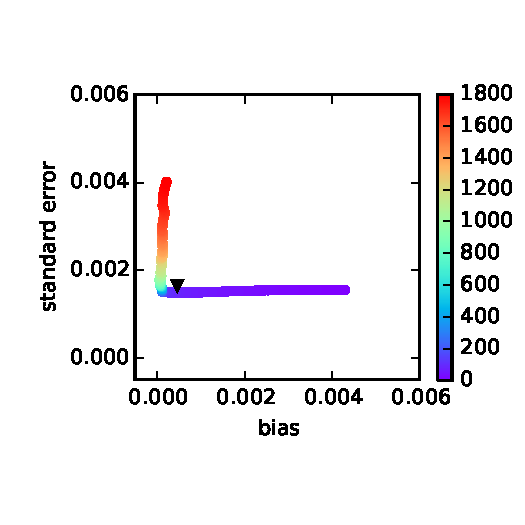
\includegraphics{argon-bias-variance.pdf}}
\caption{\label{figure:bias-variance} {\bf Bias-variance tradeoff for fixed equilibration time versus automatic equilibration time selection.} 
Trajectories of length $T = 2000 \tau$ for the argon system described in Figure~\ref{figure:burn-in-example} were analyzed as a function of equilibration time choice $t_0$, with colors denoting the value of $t_0$ (in units of $\tau$) corresponding to each plotted point.
Using 500 replicate simulations, the average bias (average deviation from true expectation) and standard deviation (random variation from replicate to replicate) were computed as a function of a prespecified fixed equilibration time $t_0$, with colors running from violet ($0~\tau$)  to red ($1800~\tau$).
As is readily discerned, the bias for small $t_0$ is initially large, but minimized for larger $t_0$.
By contrast, the standard error (a measure of variance, estimated here by standard deviation among replicates) grows as $t_0$ grows above a certain critical time (here, $\sim 100~\tau$).
If the $t_0$ that maximizes $N_\mathrm{eff}$ is instead chosen \emph{individually} for each trajectory based on that trajectory's estimates of statistical inefficiency $g_{[t_0,T]}$, the resulting bias-variance tradeoff (black triangle) does an excellent job minimizing bias and variance simultaneously, comparable to what is possible for a choice of equilibration time $t_0$ based on knowledge of the true bias and variance among many replicate estimates.
}
\end{figure}

{\bf Bias-variance tradeoff.} 
How will the simple strategy of selecting the equilibration time $t_0$ using Eq~\ref{equation:optimal-equilibration-time} work for cases where we do not know the statistical inefficiency $g$ as a function of the equilibration time $t_0$ precisely?
When all that is available is a single simulation, our best estimate of $g_{t_0}$ is derived from that simulation alone over the span $[t_0,T]$---will this affect the quality of our estimate of equilibration time?
Empirically, this does not appear to be the case---the black triangle in Figure~\ref{figure:bias-variance} shows the bias and variance contributions to the error for estimates computed over the 500 replicates where $t_0$ is individually determined from each simulation using this simple scheme based on selecting $t_0$ to maximize $N_\mathrm{eff}$ for each individual realization.
Despite not having knowledge about multiple realizations, this strategy effectively achieves a near-optimal balance between minimizing bias without increasing variance.

{\bf Overall RMS error.} 
How well does this strategy perform in terms of decreasing the \emph{overall} error $\delta \hat{A}_{[t_0,T]}$ compared to $\delta \hat{A}_{[0,T]}$?
Figure~\ref{figure:argon-rmse} compares the expected standard error (denoted $\delta \hat{A}$) as a function of a fixed initial equilibration time $t_0$ (black line with shaded region denoting 95\% confidence interval) with the strategy of selecting $t_0$ to maximize $N_\mathrm{eff}$ for each realization (red line with shaded region denoting 95\% confidence interval).
While the minimum error for the fixed-$t_0$ strategy (0.00152$\pm$0.00005) is achieved at $\sim 100~\tau$---a fact that could only be determined from knowledge of multiple realizations---the simple strategy of selecting $t_0$ using Eq.~\ref{equation:optimal-equilibration-time} achieves a minimum error of 0.00173$\pm$0.00005, only 11\% worse (compared to errors of 0.00441$\pm$0.00007, or 290\% worse, should no data have been discarded).

%%%%%%%%%%%%%%%%%%%%%%%%%%%%%%%%%%%%%%%%%%%%%%%%%%%%%%%%%%%%%%%%%%%%%%%%%%%%%%%%
% FIGURE: RMS ERROR
%%%%%%%%%%%%%%%%%%%%%%%%%%%%%%%%%%%%%%%%%%%%%%%%%%%%%%%%%%%%%%%%%%%%%%%%%%%%%%%%

\begin{figure*}[tbp]
\resizebox{\columnwidth}{!}{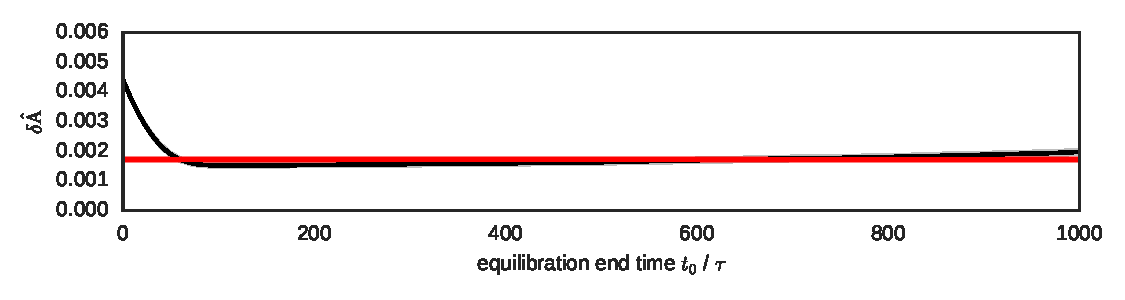
\includegraphics{argon-rmse.pdf}}
\caption{\label{figure:argon-rmse} {\bf RMS error for fixed equilibration time versus automatic equilibration time selection.} 
Trajectories of length $T = 2000 \tau$ for the argon system described in Figure~\ref{figure:burn-in-example} were analyzed as a function of fixed equilibration time choice $t_0$.
Using 500 replicate simulations, the root-mean-squared (RMS) error (Eq.~\ref{equation:rms-error}) was computed (black line) along with 95\% confidence interval (gray shading).
The RMS error is minimized for fixed equilibration time choices in the range 100--200 $\tau$.
If the $t_0$ that maximizes $N_\mathrm{eff}$ is instead chosen \emph{individually} for each trajectory based on that trajectory's estimated statistical inefficiency $g_{[t_0,T]}$ using Eq.~\ref{equation:optimal-equilibration-time}, the resulting RMS error (red line, 95\% confidence interval shown as red shading) is quite close to the minimum RMS error achieved from any particular \emph{fixed} choice of equilibration time $t_0$, suggesting that this simple automated approach to selecting $t_0$ achieves close to optimal performance.
}
\end{figure*}

%%%%%%%%%%%%%%%%%%%%%%%%%%%%%%%%%%%%%%%%%%%%%%%%%%%%%%%%%%%%%%%%%%%%%%%%%%%%%%%%
% DISCUSSION
%%%%%%%%%%%%%%%%%%%%%%%%%%%%%%%%%%%%%%%%%%%%%%%%%%%%%%%%%%%%%%%%%%%%%%%%%%%%%%%%

\section*{Discussion}
\label{section:discussion}

The scheme described here---in which the equilibration time $t_0$ is computed using Eq.~\ref{equation:optimal-equilibration-time} as the choice that maximizes the number of uncorrelated samples in the production region $[t_0,T]$---is both conceptually and computationally straightforward.
It provides an approach to determining the optimal amount of initial data to discard to equilibration in order to minimize variance while also minimizing initial bias, and does this without employing statistical tests that require generally unsatisfiable assumptions of normality of the observable of interest.
All that is needed is to save the timeseries $\{a_t\}_1^T$ of the observable $A(x)$ of interest---there is no need to store full configurations $x_t$---and post-process this dataset with a simple analysis procedure, for which we have provided a convenient Python reference implementation (see \emph{Simulation Details}).
As we have seen, this scheme empirically appears to select a practical compromise between bias and variance even when the statistical inefficiency $g$ is estimated directly from the trajectory using Eq.~\ref{equation:statistical-inefficiency-definition}.

To show that this approach is indeed general, we repeated the analysis illustrated above in Figs.~\ref{figure:burn-in-example}--\ref{figure:argon-rmse} for a different choice of observable $A(x)$ for the same liquid argon system---in this case, the reduced potential energy\footnote{Note that the \emph{reduced potential}~\cite{shirts-chodera:jcp:2008:mbar} for the isothermal-isobaric ensemble is generally defined as $u^*(x) = \beta[u(x) + p V(x)]$ to include the pressure-volume term $\beta p V(x)$, but in order to demonstrate the performance of this analysis on an observable distinct from the density---which depends on $V(x)$---we omit the $\beta p V(x)$ term in the present analysis.} $u^*(x) \equiv \beta U(x)$.
The results of this analysis are collected in Fig.~\ref{figure:reduced-potential}.
As can readily be seen, this reduced potential behaves in essentially the same way the reduced density does, and the simple scheme for automated determination of equilibration time $t_0$ from Eq.~\ref{equation:optimal-equilibration-time} does just as well.

A word of caution is necessary.
One can certainly envision pathological scenarios where this algorithm for selecting an optimal equilibration time will break down.
In cases where the simulation is not long enough to reach equilibrium---let alone collect many uncorrelated samples from it---no choice of equilibration time will bestow upon the experimenter the ability to produce an unbiased estimate of the true expectation.
Similarly, in cases where insufficient data is available for the statistical inefficiency to be estimated well, this algorithm is expected to perform poorly.
However, in these cases, the data itself should be suspect if the trajectory is not at least an order of magnitude longer than the minimum estimated autocorrelation time.

%%%%%%%%%%%%%%%%%%%%%%%%%%%%%%%%%%%%%%%%%%%%%%%%%%%%%%%%%%%%%%%%%%%%%%%%%%%%%%%%
% METHODS
%%%%%%%%%%%%%%%%%%%%%%%%%%%%%%%%%%%%%%%%%%%%%%%%%%%%%%%%%%%%%%%%%%%%%%%%%%%%%%%%

\section*{Simulation Details}
\label{section:methods}

All molecular dynamics simulations described here were performed with OpenMM 6.3~\cite{eastman:jctc:2012:openmm} (available at \href{http://openmm.org}{openmm.org}) using the Python API.
All scripts used to retrieve the software versions used here, run the simulations, analyze data, and generate plots---along with the simulation data itself and scripts for generating figures---are available on GitHub\footnote{All Python scripts necessary to reproduce this work---along with data plotted in the published version---are available at:\\
\url{http://github.com/choderalab/automatic-equilibration-detection}}.

To model liquid argon, the {\tt LennardJonesFluid} model system in the \href{http://github.com/choderalab/openmmtools}{openmmtools} package\footnote{available at \url{http://github.com/choderalab/openmmtools}} was used with parameters appropriate for liquid argon ($\sigma = $ 3.4 \AA, $\epsilon = $ 0.238 kcal/mol).
All results are reported in reduced (dimensionless) units.
Initial dense liquid geometries were generated via a Sobol' subrandom sequence~\cite{sobol:1967:ussr-comput-maths-math-phys:sobol-subrandom-sequence}, as generated by the {\tt subrandom\_particle\_positions} method in {\tt openmmtools}. 
A cubic switching function was employed, with the potential gently switched to zero over $r \in [\sigma, 3 \sigma]$, and a long-range isotropic dispersion correction accounting for this switching behavior used to include neglected contributions.
Simulations were performed using a periodic box of $N = 500$ atoms at reduced temperature $T^* \equiv k_B T / \epsilon = 0.850$ and reduced pressure $p^* \equiv p \sigma^3 / \epsilon = 1.266$ using a Langevin integrator~\cite{sivak-chodera-crooks:jpcb:2014:vvvr} with timestep $\Delta t = 0.01 \tau$ and collision rate $\nu = \tau^{-1}$, with characteristic oscillation timescale $\tau = \sqrt{m r_0^2 / 72 \epsilon}$ and $r_0 = 2^{1/6} \sigma$~\cite{liquid-argon-characteristic-timescale}.
All times are reported in multiples of the characteristic timescale $\tau$.
A molecular scaling Metropolis Monte Carlo barostat with Gaussian simulation volume change proposal moves attempted every $\tau$ (100 timesteps), using an adaptive algorithm that adjusts the proposal width during the initial part of the simulation~\cite{eastman:jctc:2012:openmm}.
Densities were recorded every $\tau$ (100 timesteps).
The true expectation $\expect{ \rho^* }$ was estimated from the sample average over all 500 realizations over [5000,10000] $\tau$.

The automated equilibration detection scheme is also available in the \href{http://pymbar.readthedocs.org/en/latest/timeseries.html}{\tt timeseries} module of the \href{http://github.com/choderalab/pymbar}{\tt pymbar} package as {\tt detectEquilibration()}, and can be accessed using the following code:

\begin{minted}[mathescape,
%               linenos,
               numbersep=5pt,
               gobble=0,
               frame=lines,
               framesep=2mm]{python}
from pymbar.timeseries import detectEquilibration
# determine equilibrated region
[t0, g, Neff_max] = detectEquilibration(A_t)
# discard initial samples to equilibration
A_t = A_t[t0:]
\end{minted}

%%%%%%%%%%%%%%%%%%%%%%%%%%%%%%%%%%%%%%%%%%%%%%%%%%%%%%%%%%%%%%%%%%%%%%%%%%%%%%%%
% STATISTICAL INEFFICIENCY
%%%%%%%%%%%%%%%%%%%%%%%%%%%%%%%%%%%%%%%%%%%%%%%%%%%%%%%%%%%%%%%%%%%%%%%%%%%%%%%%

\section*{Practical computation of statistical inefficiencies}

The robust computation of the statistical inefficiency $g$ (defined by Eq.~\ref{equation:statistical-inefficiency-definition}) for a finite timeseries $a_t$, $t = 0, \ldots, T$ deserves some comment.
There are, in fact, a variety of schemes for estimating $g$ described in the literature, and their behaviors for finite datasets may differ, leading to different estimates of the equilibration time $t_0$ using the algorithm of Eq.~\ref{equation:optimal-equilibration-time}.

The main issue is that a straightforward approach to estimating the statistical inefficiency using Eqs.~\ref{equation:integrated-autocorrelation-time-definition}--\ref{equation:autocorrelation-definition} in which the expectations are simply replaced with sample estimates causes the statistical error in the estimated correlation function $C_t$ to grow with $t$ in a manner that allows this error to quickly overwhelm the sum of Eq.~\ref{equation:integrated-autocorrelation-time-definition}.
As a result, a number of alternative schemes---generally based on controlling the error in the estimated $C_t$ or truncating the sum of Eq.~\ref{equation:integrated-autocorrelation-time-definition} when the error grows too large---have been proposed.

For stationary, irreducible, reversible Markov chains, Geyer observed that a function $\Gamma_{k} \equiv \gamma_{2k} + \gamma_{2k+1}$ of the unnormalized fluctuation autocorrelation function $\gamma_t \equiv \expect{a_i a_{i+t}} - \expect{a_i}^2$ has a number of pleasant properties (Theorem 3.1 of \cite{geyer:1992:stat-sci:practical-mcmc}): It is strictly positive, strictly decreasing, and strictly convex.
Some or all of these properties can be exploited to define a family of estimators called \emph{initial sequence methods} (see Section 3.3 of \cite{geyer:1992:stat-sci:practical-mcmc} and Section 1.10.2 of \cite{crc-mcmc-handbook}), of which the \emph{initial convex sequence} (ICS) estimator is generally agreed to be optimal, if somewhat more complex to implement.\footnote{Implementations of these methods are provided with the code distributed with this manuscript.}

All computations in this manuscript used the fast multiscale method described in Section 5.2 of \citep{chodera:jctc:2007:wham}, which we found performed equivalently well to the Geyer estimators (data not shown).
This method is related to a multiscale variant of the \emph{initial positive sequence} (IPS) method of Geyer \cite{geyer-thompson:j-royal-stat-soc-b:1992:initial-sequence-estimators}, where contributions are accumulated at increasingly longer lag times and the sum of Eq.~\ref{equation:integrated-autocorrelation-time-definition} is truncated when the terms become negative.
We have found this method to be both fast and to provide useful estimates of the statistical inefficiency, but it may not perform well for all problems.

%%%%%%%%%%%%%%%%%%%%%%%%%%%%%%%%%%%%%%%%%%%%%%%%%%%%%%%%%%%%%%%%%%%%%%%%%%%%%%%%
% FIGURE: REDUCED POTENTIAL
%%%%%%%%%%%%%%%%%%%%%%%%%%%%%%%%%%%%%%%%%%%%%%%%%%%%%%%%%%%%%%%%%%%%%%%%%%%%%%%%

\begin{figure*}[tbp]
\subfigure[\emph{Top:} Average reduced potential for relaxation from initial conditions (black solid line).
\emph{Bottom:} Cumulative averages of reduced potential with (blue solid line) and without (red dotted line) discarding some initial data to equilibration.
]{\resizebox{0.9\textwidth}{!}{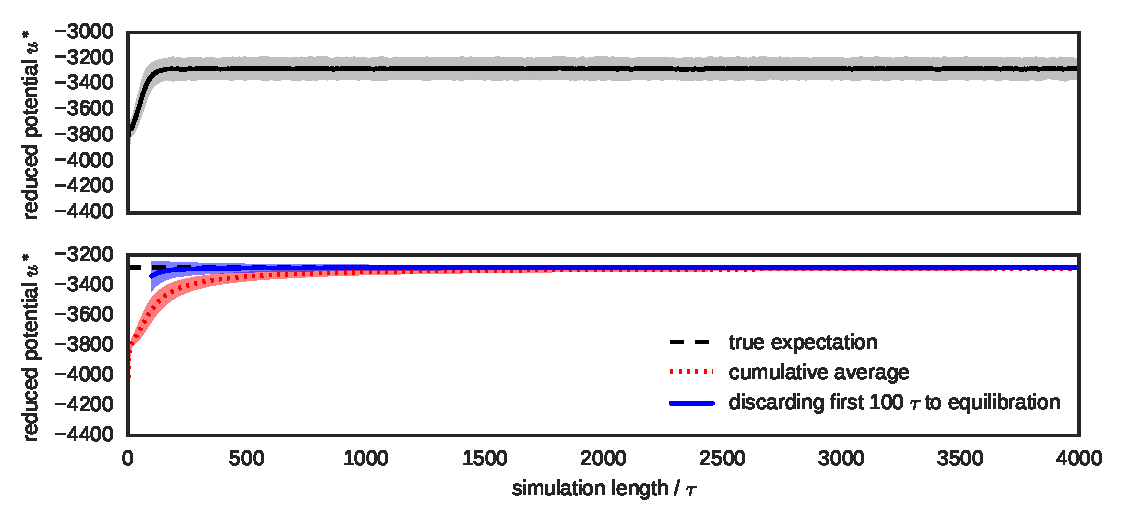
\includegraphics{argon-potential.pdf}}}
\subfigure[Statistical inefficiency $g$, effective number of uncorrelated samples $N_\mathrm{eff}$, and average of reduced potential $u^*$ omitting equilibration time $t_0$ for analysis of reduced potential.]{\resizebox{0.9\textwidth}{!}{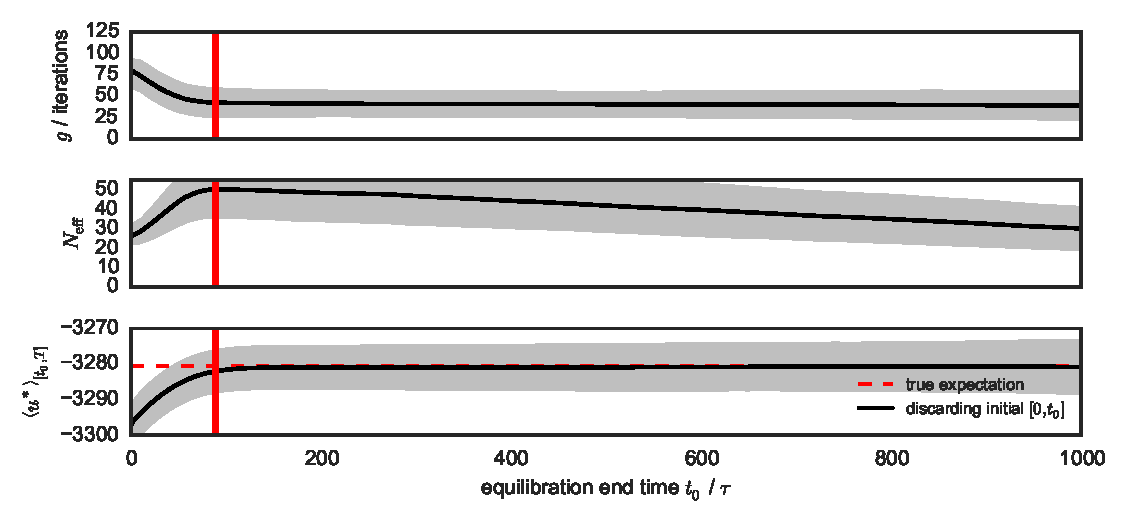
\includegraphics{argon-potential-reverse-cumulative-average.pdf}}}
\subfigure[Bias-variance tradeoff for reduced potential.]{\resizebox{0.22\textwidth}{!}{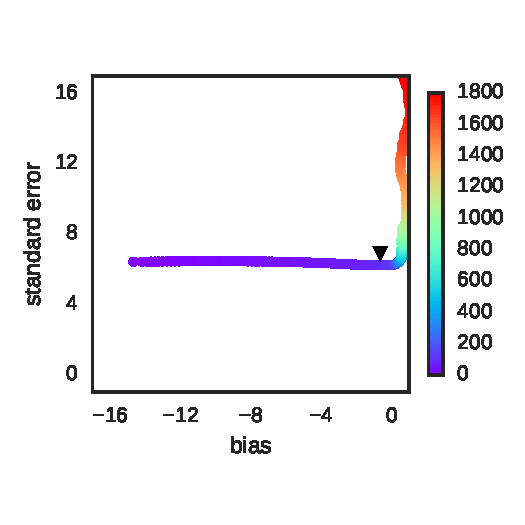
\includegraphics{argon-potential-bias-variance.pdf}}}
\subfigure[Overall RMSE error in estimate of reduced potential as a function of discarded equilibration time (black) compared with RMSE from automatic equilibration detection scheme (red line).]{\resizebox{0.77\textwidth}{!}{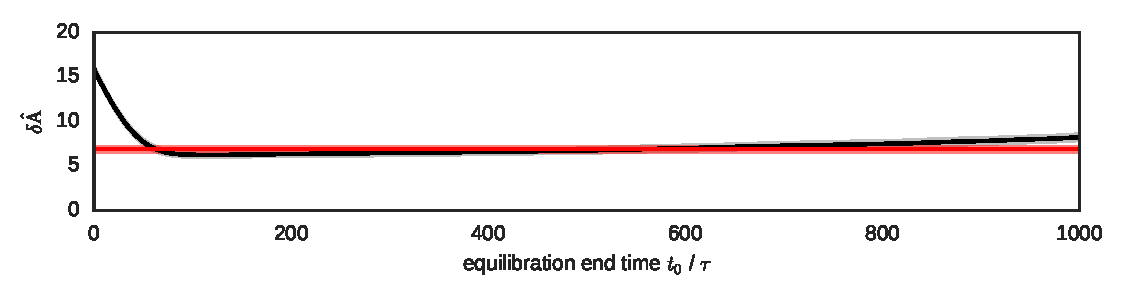
\includegraphics{argon-potential-rmse.pdf}}}

\caption{\label{figure:reduced-potential} {\bf Corresponding analysis for reduced potential energy of liquid argon system.}
The analyses of Figs.~\ref{figure:burn-in-example}--\ref{figure:argon-rmse} were repeated for the reduced potential energy $u^*(x) \equiv \beta U(x)$ of the liquid argon system.  
As with the analysis of reduced density, the simple automated determination of equilibration time $t_0$ from Eq.~\ref{equation:optimal-equilibration-time} works equivalently well for the reduced potential.
Shaded regions denote 95\% confidence interval.
}
\end{figure*}

%%%%%%%%%%%%%%%%%%%%%%%%%%%%%%%%%%%%%%%%%%%%%%%%%%%%%%%%%%%%%%%%%%%%%%%%%%%%%%%%
% ACKNOWLEDGMENTS
%%%%%%%%%%%%%%%%%%%%%%%%%%%%%%%%%%%%%%%%%%%%%%%%%%%%%%%%%%%%%%%%%%%%%%%%%%%%%%%%

\section*{Acknowledgments}

We are grateful to William C.~Swope (IBM Almaden Research Center) for his illuminating introduction to the use of autocorrelation analysis for the characterization of statistical error, as well as Michael R.~Shirts (University of Virginia), David L.~Mobley (University of California, Irvine), Michael K.~Gilson (University of California, San Diego), Kyle A.~Beauchamp (MSKCC), and Robert C.~McGibbon (Stanford University) for valuable discussions on this topic, and Joshua L.~Adelman (University of Pittsburgh) for helpful feedback and encouragement.
We are grateful to Michael K.~Gilson (University of California, San Diego), Wei Yang (Florida State University), Sabine Rei{\ss}er (SISSA, Italy), and the anonymous referees for critical feedback on the manuscript itself.
JDC acknowledges a Louis V.~Gerstner Young Investigator Award, NIH core grant P30-CA008748, and the Sloan Kettering Institute for funding during the course of this work.

%%%%%%%%%%%%%%%%%%%%%%%%%%%%%%%%%%%%%%%%%%%%%%%%%%%%%%%%%%%%%%%%%%%%%%%%%%%%%%%%
% BIBLIOGRAPHY
%%%%%%%%%%%%%%%%%%%%%%%%%%%%%%%%%%%%%%%%%%%%%%%%%%%%%%%%%%%%%%%%%%%%%%%%%%%%%%%%

%\bibliographystyle{prsty} 
%\bibliographystyle{achemso} 
\bibliography{automatic-equilibration-detection}

\end{document}